% example_rmk2
\documentclass{standalone}

\usepackage{tikz}
    
\usepackage{graphicx} % Работа с графикой \includegraphics{}
\graphicspath{{./images/img1/}} % картинки в папке ./images/img1/
    
\begin{document}
\begin{tikzpicture}
    \node[above] at (3.5,0)
        {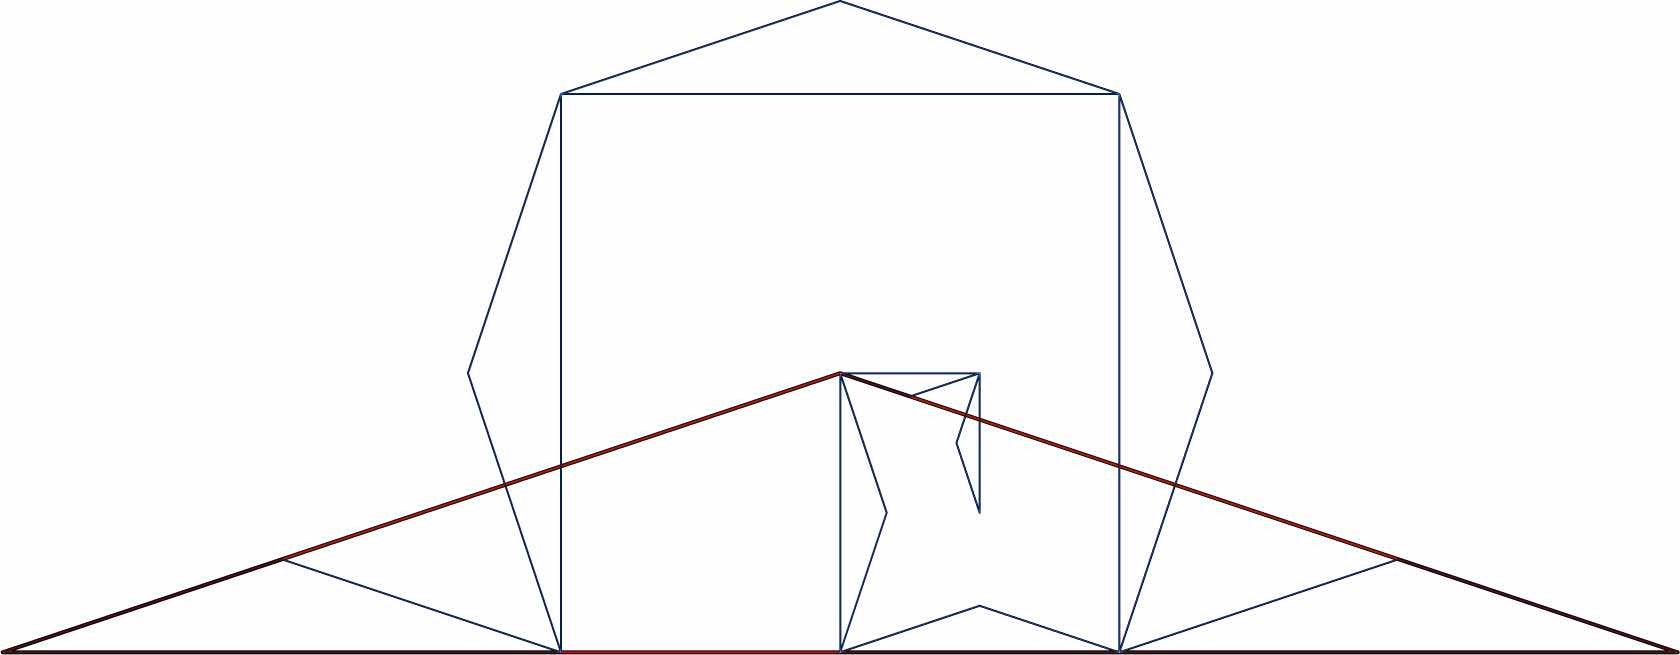
\includegraphics[width=7cm]{cntrex0.jpg}};
    \node[above] at (11,0)
       {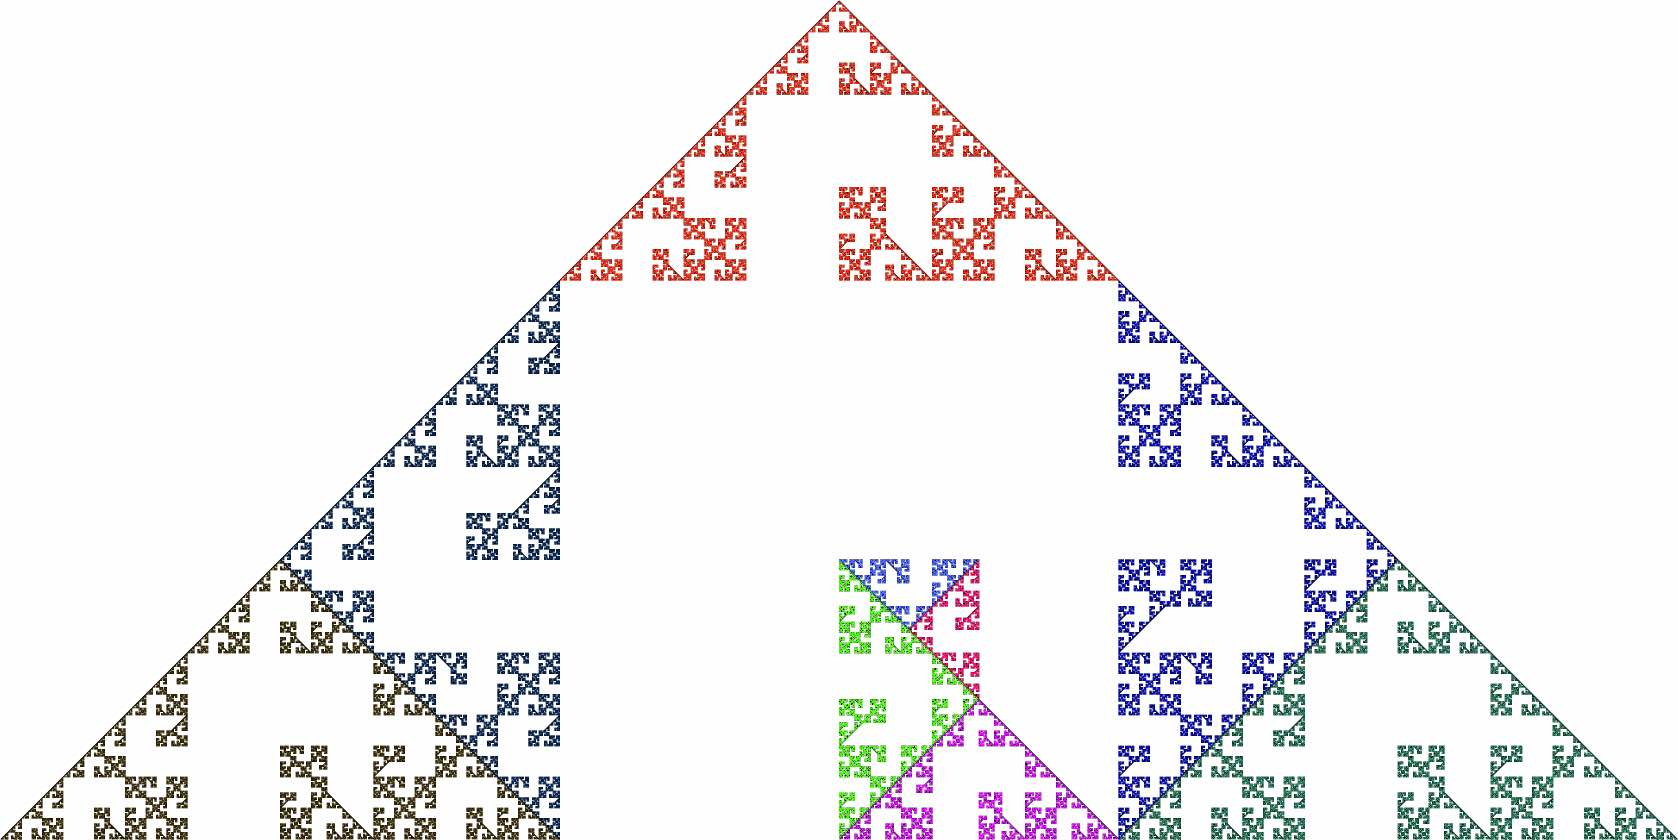
\includegraphics[width=7cm]{cntrex.jpg}}; 
    \draw 
        (1.2,-0.1) node {$P_1$} 
        (1.7,1.3)  node {$P_2$} 
        (3.5,3.1)  node {$P_3$}
        (5.3,1.3)  node {$P_4$} 
        (5.8,-0.1) node {$P_5$} 
        (4.1,-0.1) node {$P_6$} 
        (3.2,0.7)  node {$P_7$} 
        (3.8,1.5)  node {$P_8$} 
        (4.3,0.7)  node {$P_9$}
        %%%%%%%%%%%
        (8.5,-0.1)  node {$K_1$} 
        (9,2)       node {$K_2$} 
        (11,2.2)    node {$K_3$}
        (13,2)      node {$K_4$} 
        (13.5,-0.1) node {$K_5$} 
        (11.6,-0.1) node {$K_6$} 
        (10.7,0.7)  node {$K_7$} 
        (11.3,1.5)  node {$K_8$} 
        (11.8,1)    node {$K_9$};
    % \draw[help lines, green] (0,0) grid (15,4);
\end{tikzpicture}

\end{document}